Betrachtet werden die beiden Funktionen, welche in Abbildung \ref{deconvolve:1d} dargestellt sind.
\begin{figure}[h]
\centering
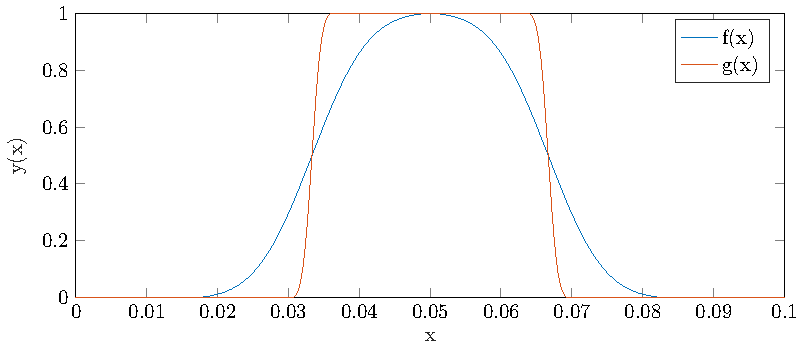
\includegraphics[width=0.9\textwidth]{./papers/deconvolve/pictures/1d.pdf}
\caption{Funktionen für die eindimensionalen Versuche\label{deconvolve:1d}}5
\end{figure}
Eine stetige Wavelet-Transformation von $f(x)$ ist in \ref{deconvolve:y1_cwt} abgebildet.
Lässt man nur bestimmte Dilatationen $a$ bzw. die orangen \glqq Zeilen\grqq{} der stetigen Transformation zu, werden die Level der diskreten Transformation sichtbar.
Jedes Level tiefer wird das Wavelet \glqq halbiert\grqq{} und somit die Auflösung höher.
Hier sind der Übersicht halber nur die Level 7-13 eingezeichnet. 
Die stetige Transformation dient auch nur zur Visualisierung, für die eigentliche Umsetzung wird nur noch mit der diskreten Transformation auf den Level 1-13 gearbeitet.

Die Koeffizienten der diskreten Transformation von $f(x)$ werden als $cf_k$ bezeichnet wobei der Index $k\in[1,2,...,13]$ für das jeweilige Level steht.
Die Koeffizienten von $g(x)$ werden analog dazu $cg_k$ genannt.
\begin{figure}[h]
\centering
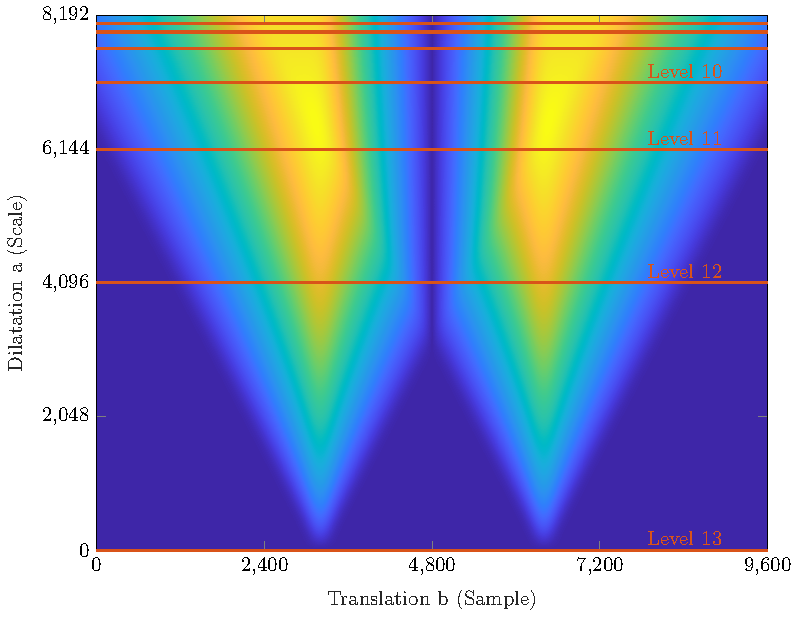
\includegraphics[width=0.9\textwidth]{./papers/deconvolve/pictures/y1_cwt.pdf}
\caption{CWT von $f(x)$\label{deconvolve:y1_cwt}}
\end{figure}

Kann nun eine Beziehung zwischen den Wavelet-Koeffizienten von $f(x)$ und $g(x)$ erkannt werden?
Die Hoffnung ist, diesen Zusammenhang als Funktion zu formulieren die $cf_k$ als Input nimmt und eine Menge an Koeffizienten zurück gibt, welche den $cg_k$ ähnlich ist.
Im Idealfall kann man also eine Funktion $s(cf_k)$ so konstruieren dass
$$cg_k = s(cf_k)$$
oder zumindest
$$cg_k \approx s(cf_k).$$

Die Rücktransformation mit den manipulierten $cf_k$ sollte dann eine Funktion liefern, welche $g(x)$ nahe kommt.
Bei Erfolg hätte man also eine Methode erarbeitet, welche aus der \glqq unscharfen\grqq{} $f(x)$ eine etwas \glqq schärfere\grqq{} Funktion $g(x)$ macht. 

\subsection{Koeffizienten manipulieren}
Abbildung \ref{deconvolve:level1} zeigt die Koeffizienten des ersten Levels der Funktionen $f(x)$ und $g(x)$ aus dem vorherigen Abschnitt, welche beide 9600 Samples lang sind.
\begin{figure}[h]
\centering
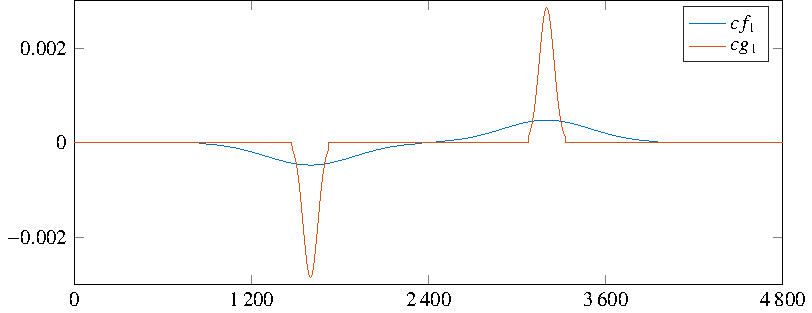
\includegraphics[width=0.9\textwidth]{./papers/deconvolve/pictures/level/level1.pdf}
\caption{Level 1 unverändert\label{deconvolve:level1}}
\end{figure}

Nun wird mit einer geeigneten Manipulation der Koeffizienten $cf_k$ versucht, die blauen Koeffizienten so anzupassen, bis sie den orangen möglichst ähnlich sind.

Man erkennt klar, dass die $cf_1$, also die Koeffizienten des ersten Level der Funktion $f(x)$ unter einer gewissen Schwelle abgeschwächt und darüber überproportional verstärkt werden müssen.
Die Funktion
$$s(cf_k) = \left( \frac{cf_k}{m}\right)^\alpha$$
ist hierfür ein vielversprechender Ansatz.
Der Parameter $m$ ist hierbei ebendiese Schwelle und mit $\alpha$ kann die Verstärkung bestimmt werden.
Wird aber $m$ sehr klein gewählt, so wird der Ausdruck in der Klammer grösser und mit der darauffolgenden Potenz $\alpha$ explodiert der Output dann förmlich.
Um dies auszugleichen muss nochmals mit $m$ multipliziert werden, wir erhalten also
$$s(f_k) = m\cdot \left( \frac{cf_k}{m}\right)^\alpha.$$
Ein Problem stellen hier aber noch negative $cf_k$ dar. In diesem Fall kann nur mit ganzzahligen Potenzen gearbeitet werden, da man sonst komplexe Lösungen erhält, welche für diese Anwendung nicht brauchbar sind.
Um dies zu Umgehen muss nur der Betrag von $cf_k$ gebildet, und deren Vorzeichen aber noch mit der Signumfunktion mitgenommen werden.
Somit erhalten wir eine Funktion
\begin{align}
s(cf_k)=m\cdot \left(\frac{|cf_k|}{m}\right)^{\alpha}\cdot \text{sign}(cf_k), \qquad m,\alpha\in\mathbb{R}
\label{deconvolve:funktion}
\end{align}
als Beziehung zwischen der \glqq unscharfen\grqq{} und \glqq scharfen\grqq{} Menge an Koeffizienten.

Abbildung \ref{deconvolve:function} zeigt unsere Funktion aus \eqref{deconvolve:funktion} mit $m=0.75$, verschiedenen $\alpha$ und der Variable $cf_k\in[-1.5;1.5]$.
Gut erkennbar ist darin, wie mit dem Parameter $\alpha$ die Verstärkung justiert werden kann.
Bei $\alpha = 1$ werden die Koeffizienten einfach übernommen.
Auch die Wirkung von $m$ wird klar.
Bei $-0.75$ und $0.75$ werden die Kurven fixiert.
\begin{figure}[h]
\centering
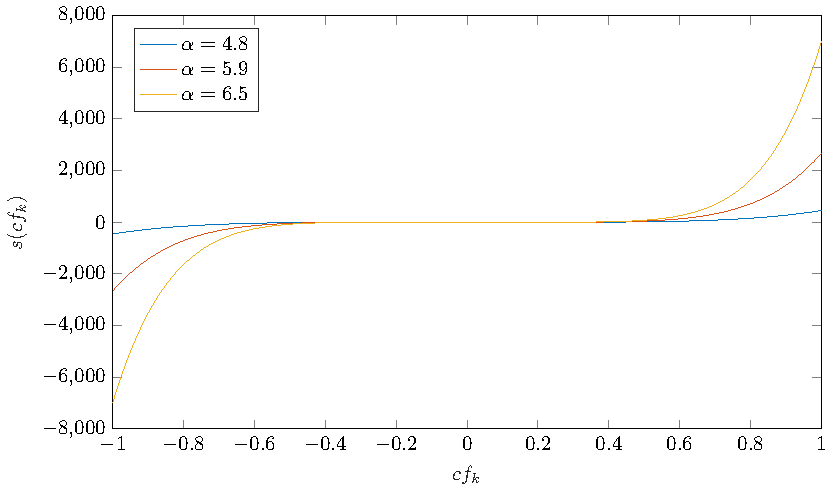
\includegraphics[width=0.9\textwidth]{./papers/deconvolve/pictures/function.pdf}
\caption{Funktion $s(cf_k)$\label{deconvolve:function}}
\end{figure}

Nun soll diese Funktion auf wenn möglich alle verschiedenen Level unserer Wavelet-Koeffizienten angewendet werden.
Für $m$ kann genau der Schnittpunkt zwischen den beiden Kurven in Abbildung \ref{deconvolve:level1} gewählt werden.
$\alpha$ wird dann so bestimmt, dass die Spitze der blauen Kurve nach der Manipulation mit derjenigen der orangen zusammenfällt.
\begin{figure}[h]
\centering
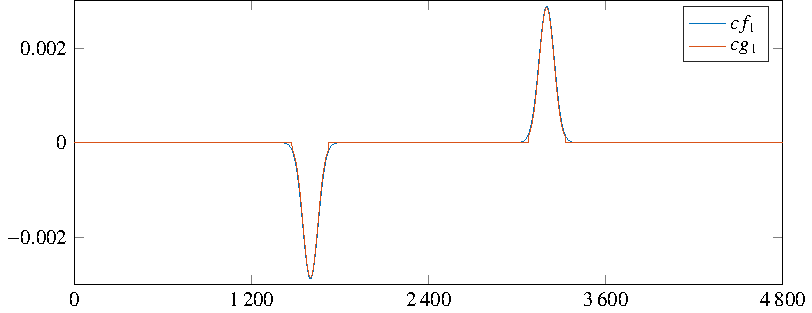
\includegraphics[width=0.9\textwidth]{./papers/deconvolve/pictures/level/level1_n.pdf}
\caption{Level 1 mit veränderten $cf_1$\label{deconvolve:level1_n}}
\end{figure}

Abbildung \ref{deconvolve:level1_n} zeigt die Funktion \eqref{deconvolve:funktion} wiederum auf das erste Level angewendet.
Der unterschied zwischen den beiden Kurven ist nur noch schwach erkennbar, die Manipulation scheint auf diesem Level also erfolgreich verlaufen zu sein.

\subsection{Koeffizienten auf höheren Level}

Mit entsprechenden $m$ und $\alpha$ soll nun gleich auf den anderen Level vorgegangen werden.
Abbildung \ref{deconvolve:level5} zeigt Level 5 vor und nach der Koeffizientenmanipulation.
\begin{figure}[h]
\centering
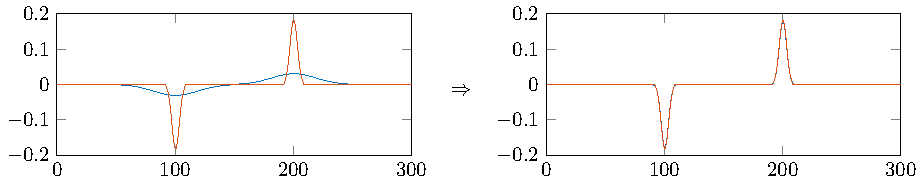
\includegraphics[width=0.9\textwidth]{./papers/deconvolve/pictures/level/level5.pdf}
\caption{Level 5 vorher und nachher\label{deconvolve:level5}}
\end{figure}

Auf diesem Level scheint alles noch wie erwünscht zu funktionieren.
Jeden Schritt höher kommen aber erwartungsgemäss weniger (halb so viele) Koeffizienten dazu.
Waren es im ersten noch 4800 sind es nun im fünften nur noch 300.
Auf dem Level 13 sind es dann nur noch zwei.
Deswegen wird es immer schwerer, die beiden Freiheitsgrade $m$ und $\alpha$ so zu wählen, dass noch eine Annäherung von $cf_k$ an $cg_k$ resultiert.
Mit dieser Beispielfunktion $f(x)$ war es möglich mit der Funktion aus \eqref{deconvolve:funktion} bis auf das Level 12 eine Verbesserung zu erreichen.

\subsection{Ergebnis}
Abbildung \ref{deconvolve:result_1d} zeigt unsere ursprüngliche Funktion $f_1(x)$.
Dessen Wavelet-Koeffizienten $cf_k$ wurden dann mit der oben beschriebenen Methode bearbeitet, was nach der Rücktransformation zu $f_2(x)$ führt.
Verglichen mit $f_1(x)$, ist $f_2(x)$ deutlich näher an $g(x)$ gerückt.
\begin{figure}[h]
\centering
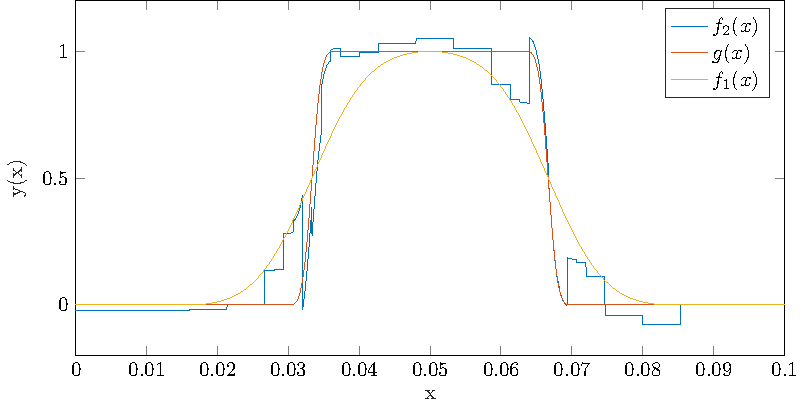
\includegraphics[width=0.9\textwidth]{./papers/deconvolve/pictures/result_1d.pdf}
\caption{Rücktransformation\label{deconvolve:result_1d}}
\end{figure}

In der Nähe des Randes hat sich die Steilheit tatsächlich vergrössert, allerdings sind weiter weg von diesem Rand zusätzliche Artefakte hinzugekommen.
Um dies besser zu verstehen wird an dieser Stelle die stetige Wavelet-Transformation zur Hilfe genommen.

In Abbildung \ref{deconvolve:cwt} sind diese ersichtlich.
Ein Vergleich der CWT von $g(x)$ und $f_1(x)$ zeigt, dass bei $f_1(x)$ \glqq Masse\grqq{} in die beiden Spitzen also nach unten verschoben werden muss.
Dies ist mit der angewandten Methode natürlich nur beschränkt möglich, da ja jedes Level einzeln behandelt wird.
Die so erzeugten Artefakte sind bei der stetigen Transformation von $f_2(x)$ als vertikale Striche in der unteren Hälfte erkennbar.
Wie gut man wieder zum Original zurückgekommen ist, sieht man noch deutlicher in der Abbildung mit der Differenz.
Auch hier erkennt man die starken Abweichungen in der unteren Hälfte.
Sie werden also von den tieferen Level bzw. Wavelets mit grosser \glqq Wellenlänge\grqq{} verursacht, welche schwer zu Manipulieren sind.
\begin{figure}[h]
\centering
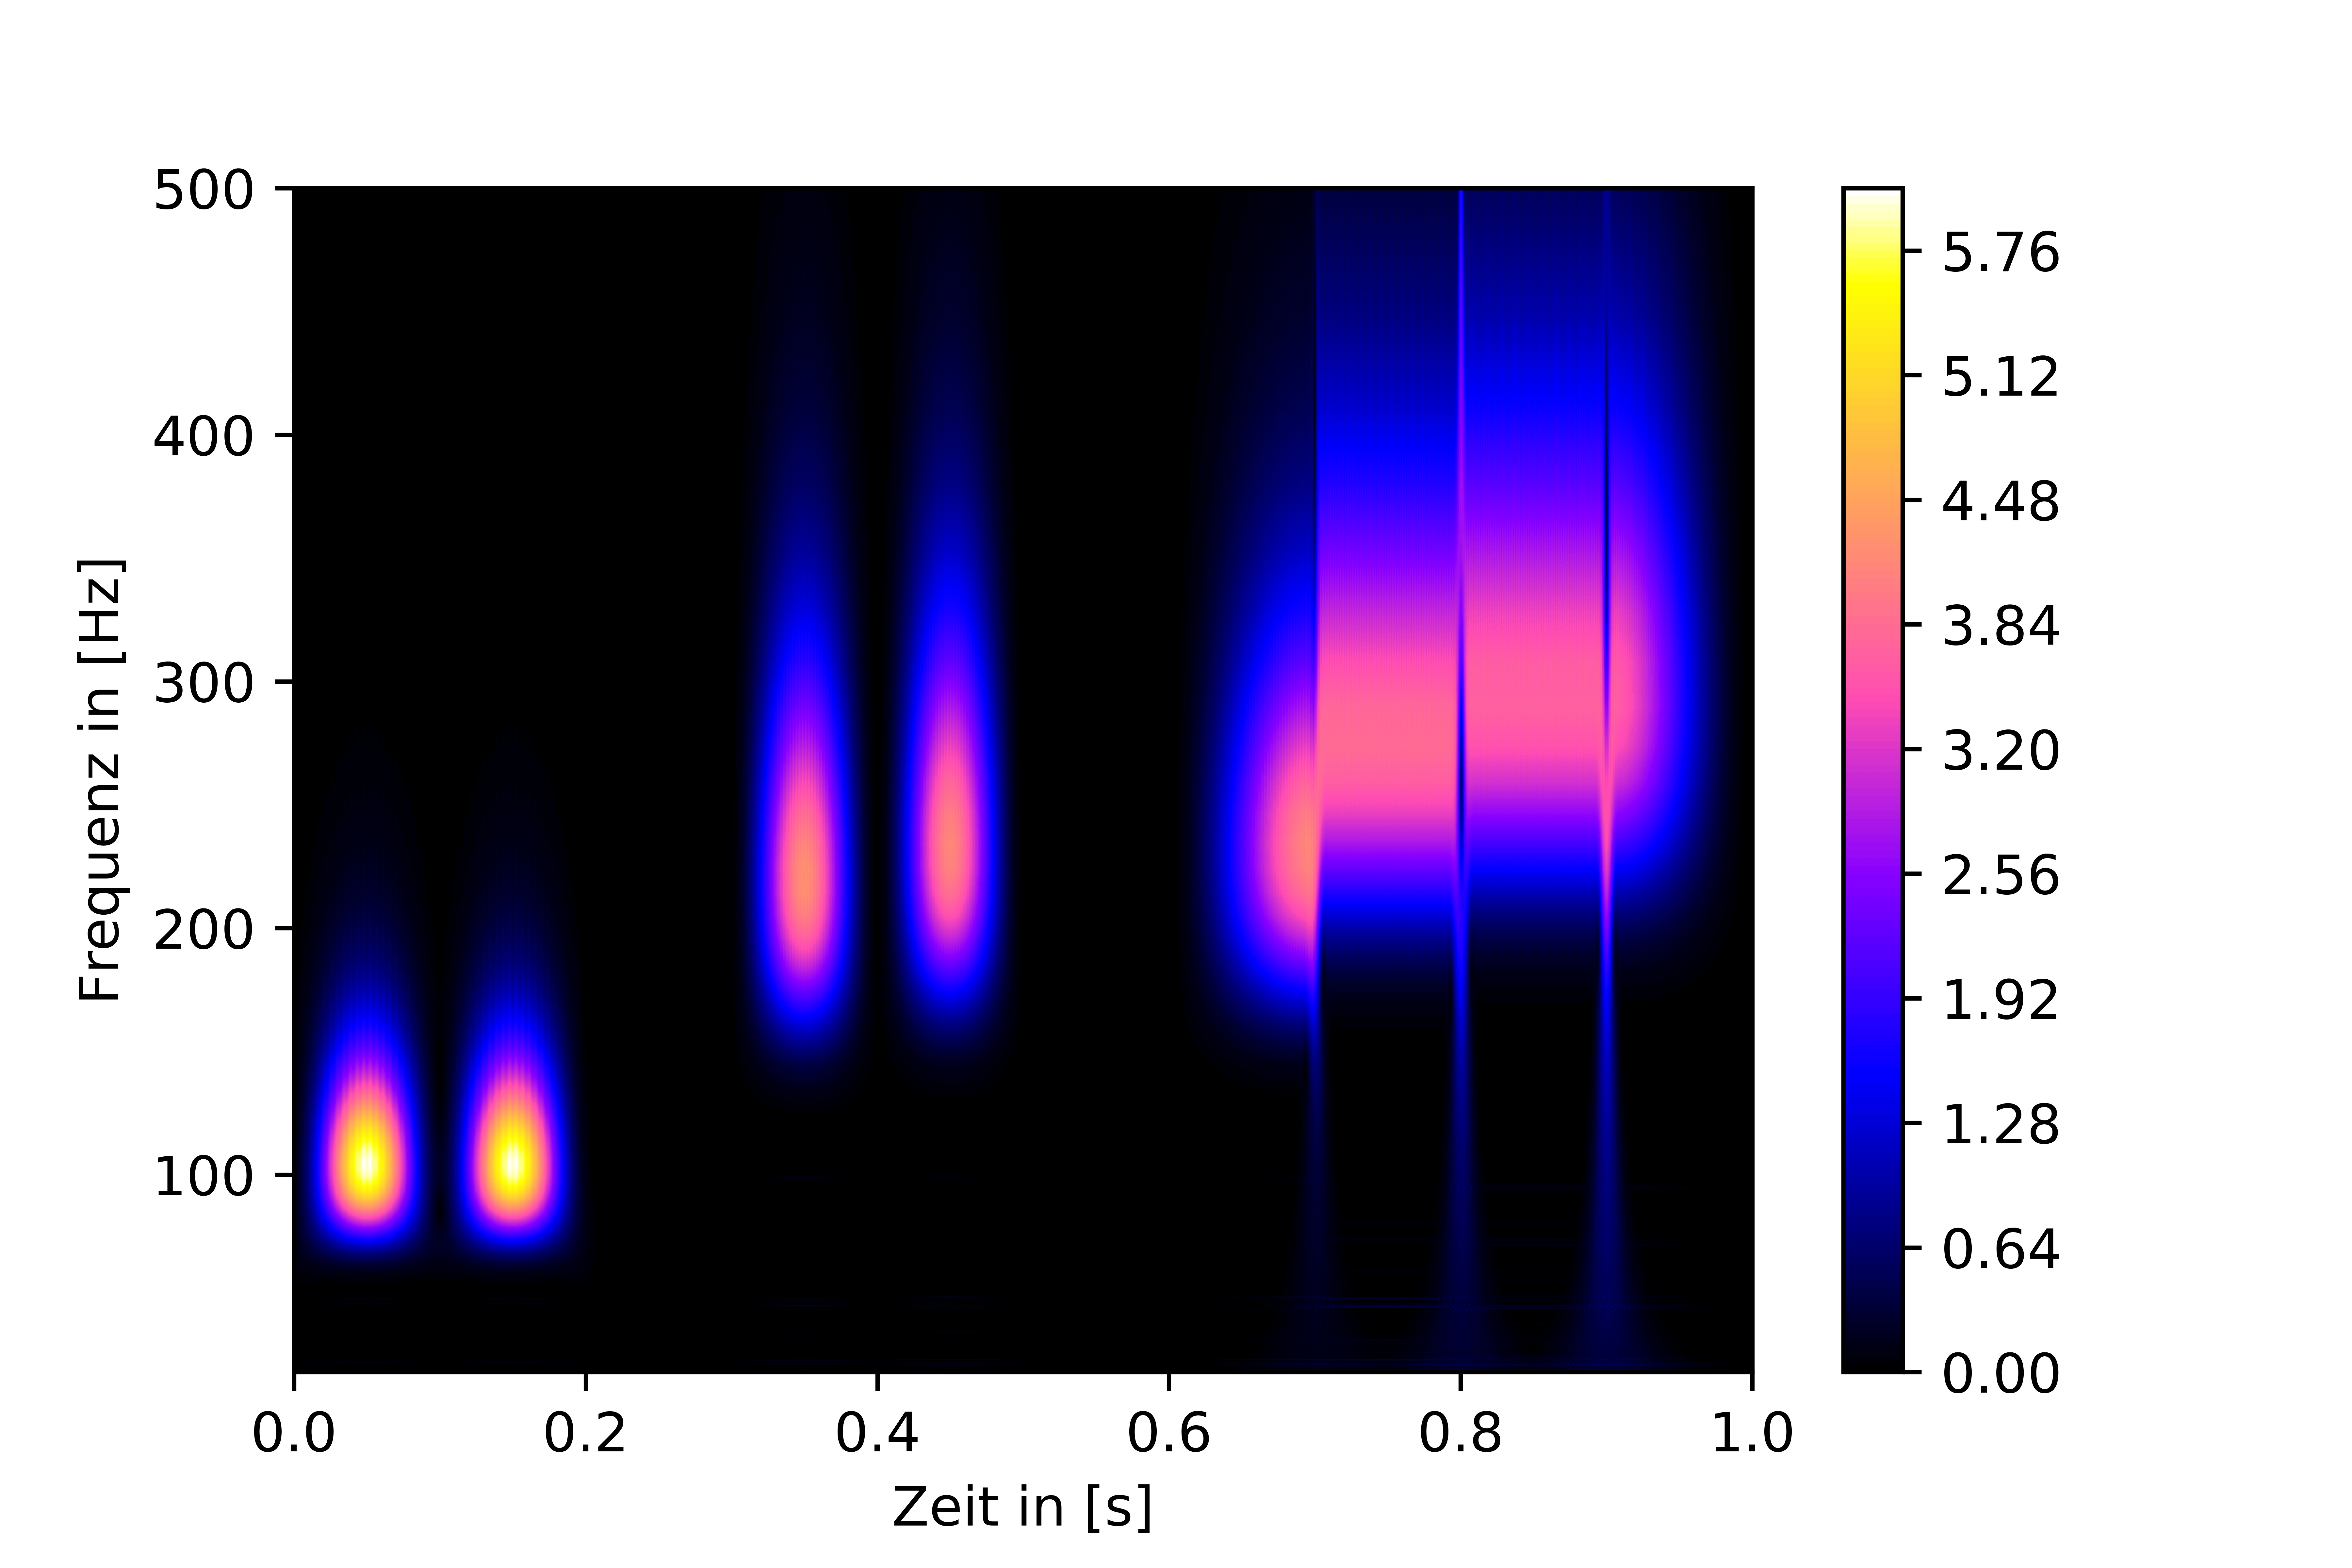
\includegraphics[width=0.9\textwidth]{./papers/deconvolve/pictures/cwt.pdf}
\caption{stetige Transformationen\label{deconvolve:cwt}}
\end{figure}
